\section{Python Exercise: DTFT Approximation using DFT}\label{sec:p6}
Figure \ref{fig:p6-1-200}-\ref{fig:p6-5-200} show the output with $M=200$. The runtime for \texttt{dtft\_approx} is 0.1s and \texttt{eq\_dtft\_approx} is 0.0005s. Figure \ref{fig:p6-1-5000}-\ref{fig:p6-5-5000} show the output with $M=5000$. The runtime for \texttt{dtft\_approx} is 2.7s and \texttt{eq\_dtft\_approx} is still 0.0005s. \texttt{dtft\_approx}'s runtime significantly increases with $M=5000$; however, $M$ does not affect \texttt{eq\_dtft\_approx} because it is implemented using \texttt{fft}.

\begin{figure}[htbp]
	\centering
	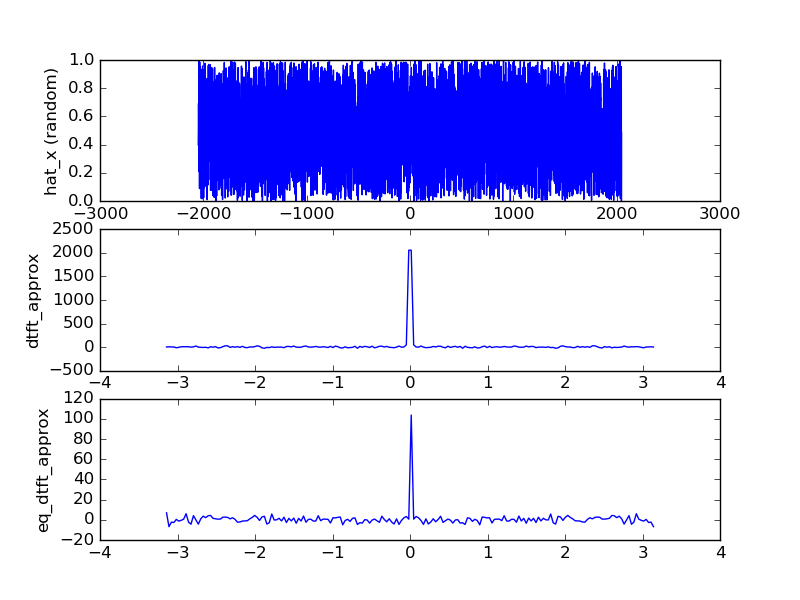
\includegraphics[width=0.8\textwidth]{images/p6-1-200}
	\caption{Random signal with $M=200$}
	\label{fig:p6-1-200}
\end{figure}

\begin{figure}[htbp]
	\centering
	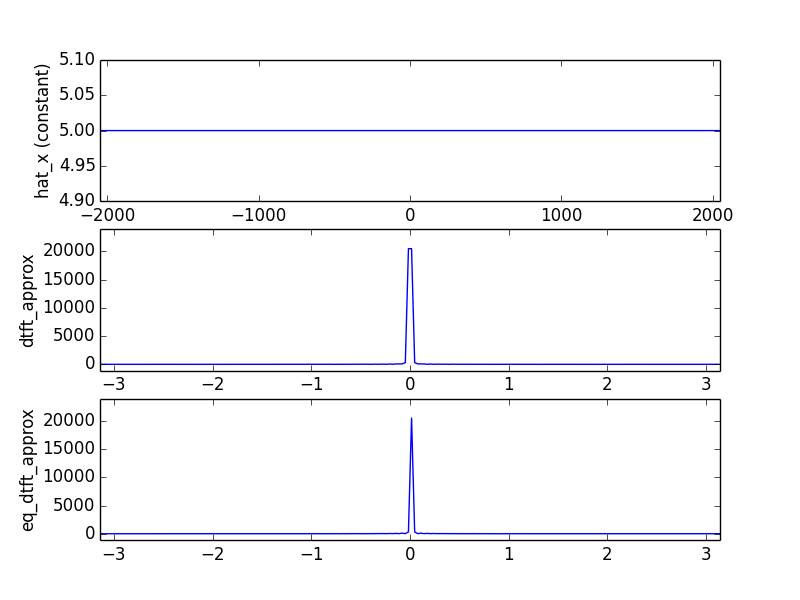
\includegraphics[width=0.8\textwidth]{images/p6-2-200}
	\caption{Constant signal with $M=200$}
	\label{fig:p6-2-200}
\end{figure}

\begin{figure}[htbp]
	\centering
	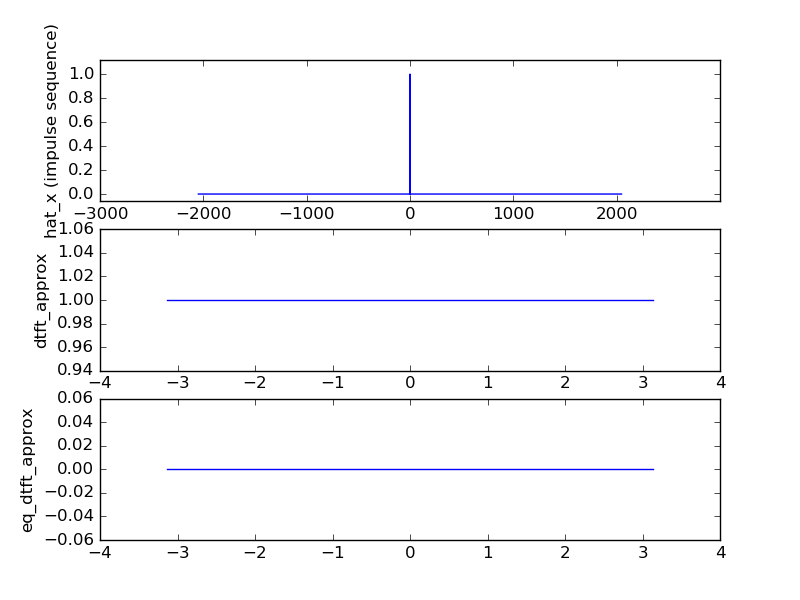
\includegraphics[width=0.8\textwidth]{images/p6-3-200}
	\caption{Impulse signal ($x[n] = \delta[n]$) with $M=200$}
	\label{fig:p6-3-200}
\end{figure}

\begin{figure}[htbp]
	\centering
	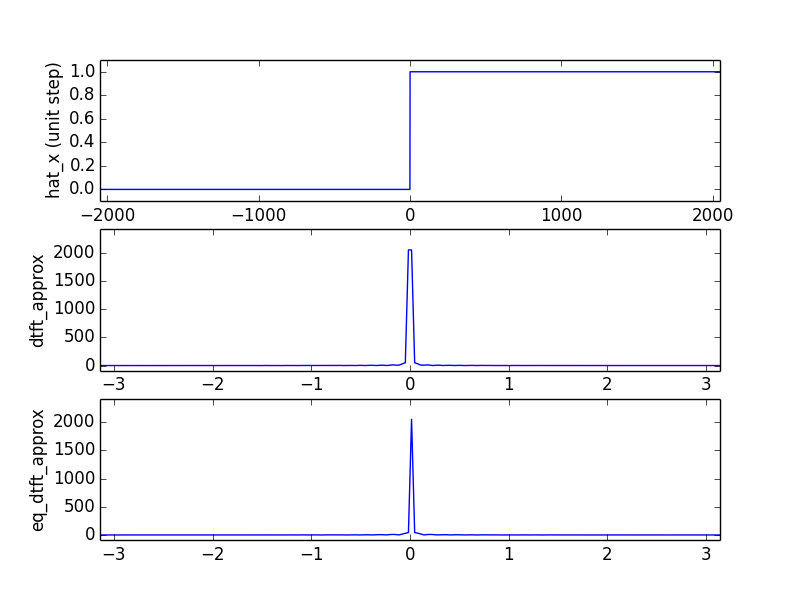
\includegraphics[width=0.8\textwidth]{images/p6-4-200}
	\caption{Unit step signal ($x[n]=u[n]$) with $M=200$}
	\label{fig:p6-4-200}
\end{figure}

\begin{figure}[htbp]
	\centering
	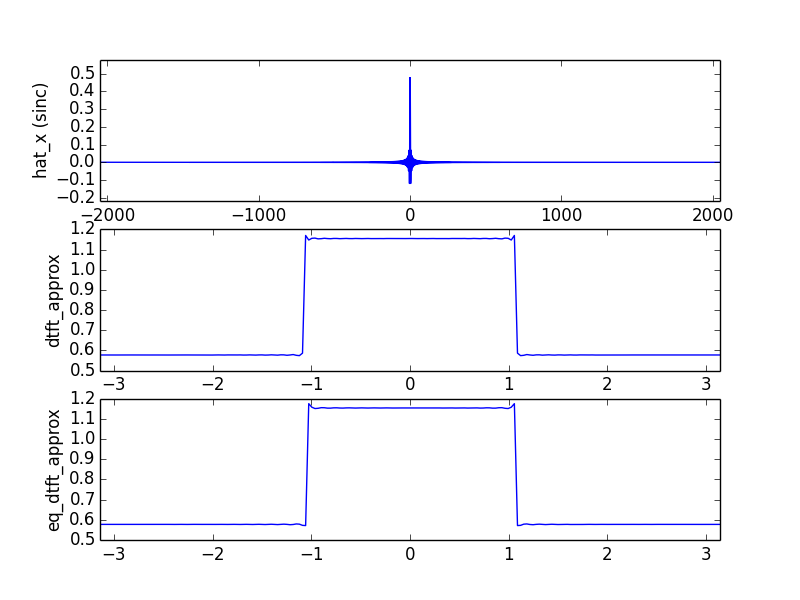
\includegraphics[width=0.8\textwidth]{images/p6-5-200}
	\caption{$x[n] = \sqrt{3}\frac{\sin(\frac{\pi n}{3})}{\pi n}$ with $M=200$}
	\label{fig:p6-5-200}
\end{figure}




\begin{figure}[htbp]
	\centering
	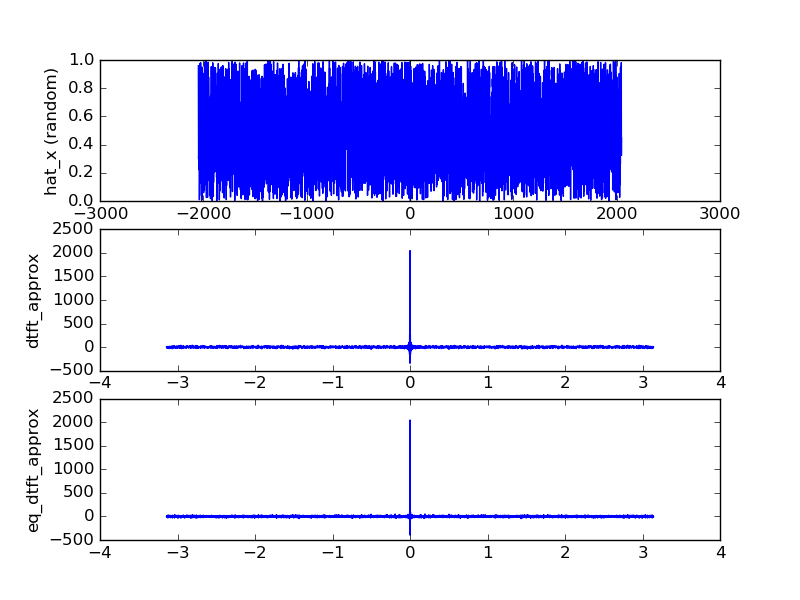
\includegraphics[width=0.8\textwidth]{images/p6-1-5000}
	\caption{Random signal with $M=5000$}
	\label{fig:p6-1-5000}
\end{figure}

\begin{figure}[htbp]
	\centering
	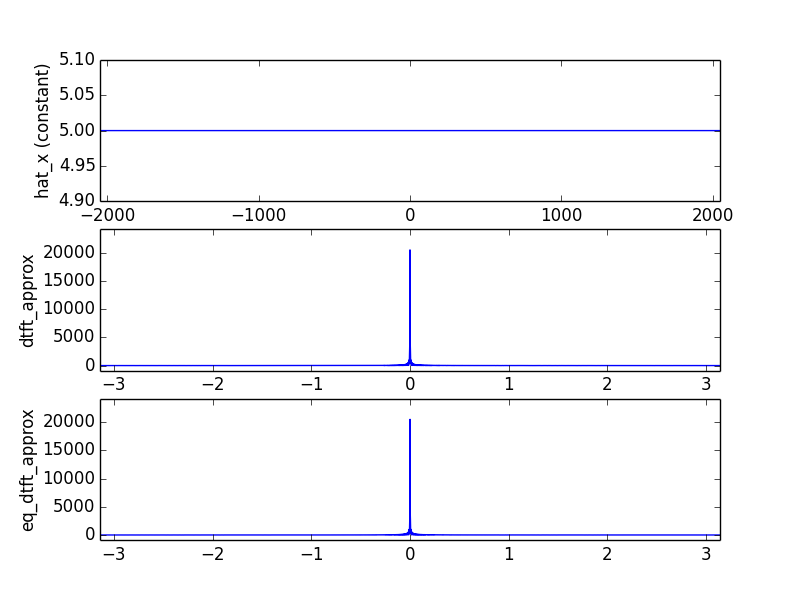
\includegraphics[width=0.8\textwidth]{images/p6-2-5000}
	\caption{Constant signal with $M=5000$}
	\label{fig:p6-2-5000}
\end{figure}

\begin{figure}[htbp]
	\centering
	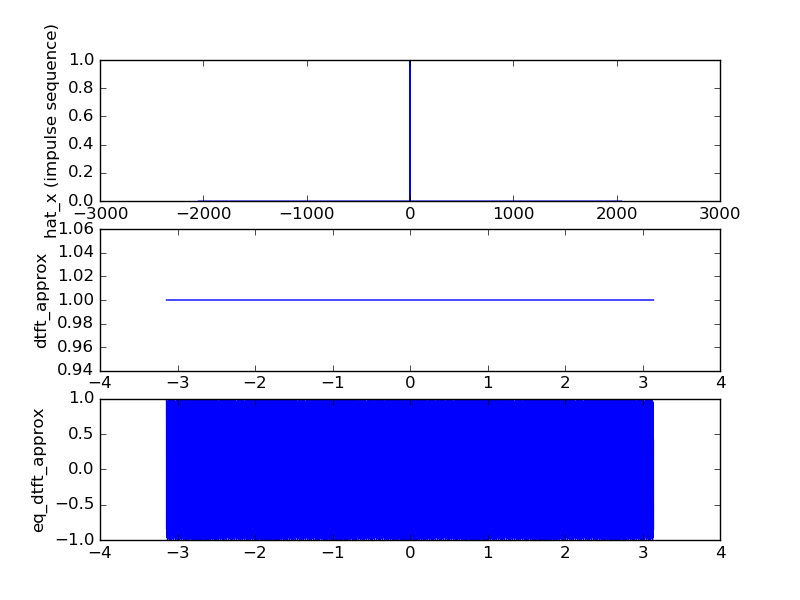
\includegraphics[width=0.8\textwidth]{images/p6-3-5000}
	\caption{Impulse signal ($x[n] = \delta[n]$) with $M=5000$}
	\label{fig:p6-3-5000}
\end{figure}

\begin{figure}[htbp]
	\centering
	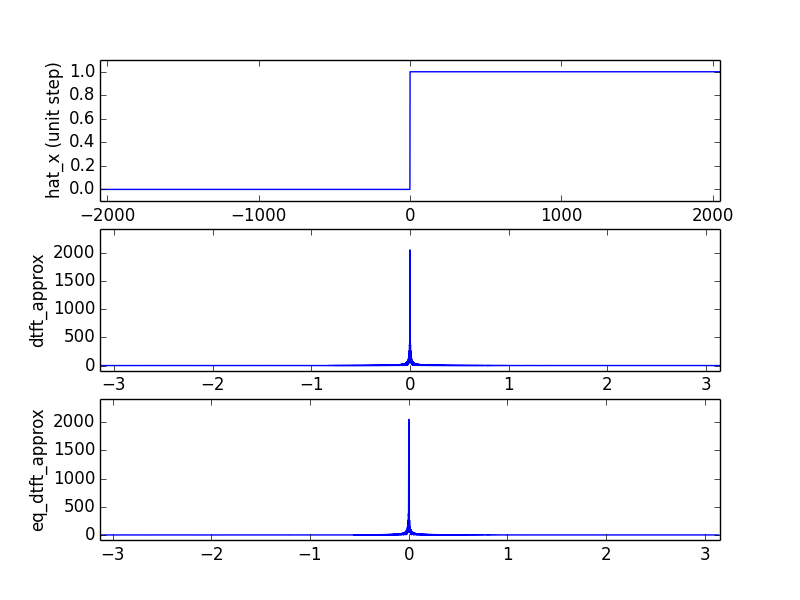
\includegraphics[width=0.8\textwidth]{images/p6-4-5000}
	\caption{Unit step signal ($x[n]=u[n]$) with $M=5000$}
	\label{fig:p6-4-5000}
\end{figure}

\begin{figure}[htbp]
	\centering
	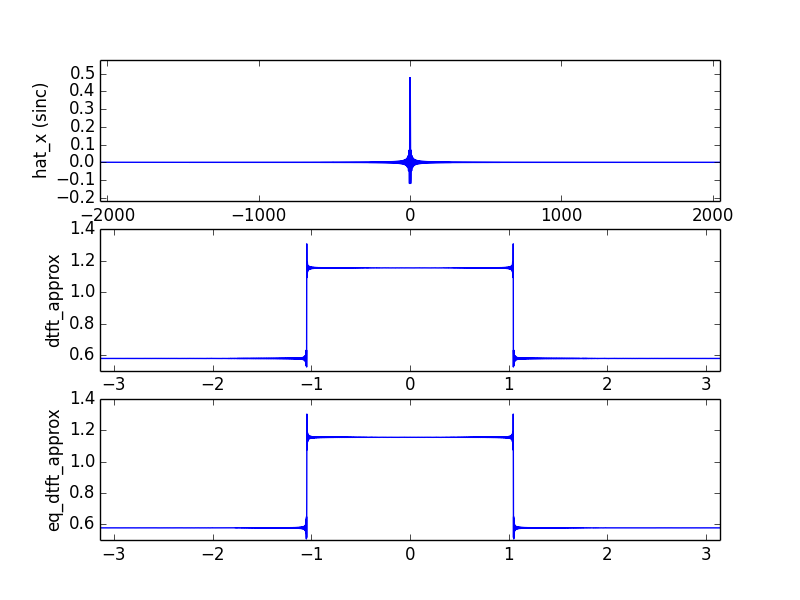
\includegraphics[width=0.8\textwidth]{images/p6-5-5000}
	\caption{$x[n] = \sqrt{3}\frac{\sin(\frac{\pi n}{3})}{\pi n}$ with $M=5000$}
	\label{fig:p6-5-5000}
\end{figure}